\documentclass{article}
\usepackage{ctex}
\usepackage{graphicx}
\usepackage{amsmath}
\usepackage{geometry}
\geometry{a4paper, left=2cm, right=2cm, top=2cm, bottom=2cm}
\title{傅里叶逼近误差分析实验报告}
\author{刘行 PB22000150}
\date{\today}

\begin{document}
\maketitle

	\section{实验背景}
		本实验旨在通过北太天元编程实现连续傅里叶级数与离散傅里叶变换的逼近, 并分析两种方法在不同截断阶数 $N$ 下的逐点误差表现. 研究对象为函数

		\begin{equation*}
			u(x)=\frac{1}{5-4\cos(x)} \quad \text{和} \quad v(x)=\sin\left(\frac{x}{2}\right), \quad x\in \left[0,\frac{\pi}{2}\right].
		\end{equation*}

		通过构造傅里叶级数逼近 $P_N u(x)$ 与离散傅里叶逼近 $I_N u(x)$, 研究其误差随截断阶数 $N$ 变化的规律, 从而深入理解傅里叶级数在函数逼近中的理论与实际效果.

	\section{实验原理}
		\subsection{连续傅里叶级数逼近}
			给定周期为 $2\pi$ 的函数 $u(x)$, 其傅里叶系数定义为

			\begin{equation*}
				\hat{u}_n = \frac{1}{2\pi}\int_{0}^{2\pi} u(x)e^{-inx}\,dx.
			\end{equation*}

			取系数 $n=-N/2, -N/2+1, \dots, N/2$ 后, 构造傅里叶级数近似为

			\begin{equation*}
				P_N u(x)=\sum_{n=-N/2}^{N/2}\hat{u}_n e^{inx}.
			\end{equation*}

		\subsection{离散傅里叶变换逼近}
			利用在区间 $[0,2\pi)$ 上均匀分布的 $N$ 个采样点 $\{x_j\}$, 定义离散傅里叶系数为

			\begin{equation*}
				\tilde{u}_n=\frac{1}{\tilde{C}_nN}\sum_{j=0}^{N-1} u(x_j)e^{-inx_j}, \quad n=-N/2,\dots,N/2. \quad
				\tilde{C}_n = \left\{
				\begin{array}{lr}
					2 & \left\lvert n \right\rvert = \frac{N}{2} \\
					1 & \left\lvert n \right\rvert \leq \frac{N}{2}
				\end{array}\right.
			\end{equation*}

			离散傅里叶逼近表示为

			\begin{equation*}
				I_N u(x)=\sum_{n=-N/2}^{N/2}\tilde{u}_n e^{inx}.
			\end{equation*}

	\section{代码思路}
		实验代码采用模块化设计, 主要包括以下模块:
		\begin{enumerate}
			\item \textbf{傅里叶系数计算:} 分别实现 \texttt{compute\_fourier\_coefficients} 和 \texttt{compute\_dft\_coefficients} 两个函数, 前者利用数值积分计算连续傅里叶系数, 后者利用离散点求和计算离散傅里叶系数. 
			\item \textbf{函数重构:} 利用计算得到的傅里叶系数, 通过 \texttt{reconstruct\_function} 函数重构出逼近函数 $P_N u(x)$ 或 $I_N u(x)$.
			\item \textbf{误差计算与绘图:} 对不同截断阶数 $N$ (取值分别为 4, 8, 16, 32, 64), 计算真实函数与逼近函数之间的逐点误差, 并利用 \texttt{plot\_error} 函数绘制误差对比图. 
		\end{enumerate}

	\section{实验结果}
		在实验中, 我们分别对函数 $u(x)$ 与 $v(x)$, 在不同的截断阶数 $N$ 下生成误差对比图. 图示展示了 $N=4,8,16,32,64$ 时, 连续傅里叶逼近 $P_N$(红线)与离散傅里叶逼近 $I_N$(蓝线)的逐点误差. 图表在实验报告的最后.

	\section{实验结论}
		\begin{itemize}
			\item 随着截断阶数 $N$ 的增加, 无论是连续傅里叶逼近 $P_N f(x)$ 还是离散傅里叶逼近 $I_N f(x)$, 其误差均显著降低. 这表明傅里叶级数在逼近周期函数方面具有较好的收敛性.
			\item 对于函数 $u(x)=\frac{1}{5-4\cos(x)}$, 其傅里叶级数收敛较快, 离散傅里叶逼近在较低的 $N$ 值时存在较大误差, 但随着 $N$ 增大, 两种方法的逼近效果趋于一致.
			\item 对于函数 $v(x)=\sin\left(\frac{x}{2}\right)$, 由于其频谱较为简单, 连续与离散傅里叶逼近均表现出较好的逼近效果, 且误差随 $N$ 增加逐步减小.
			\item 所有生成的误差图均印证了随着采样点数(或截断阶数)的增加, 逼近误差会显著降低, 从而验证了傅里叶逼近的理论分析. 实验也提醒我们, 在实际应用中应根据具体问题选择合适的 $N$ 值以达到预期的逼近精度.
		\end{itemize}

	\section{图表}

		\begin{figure}[htbp]
			\centering
			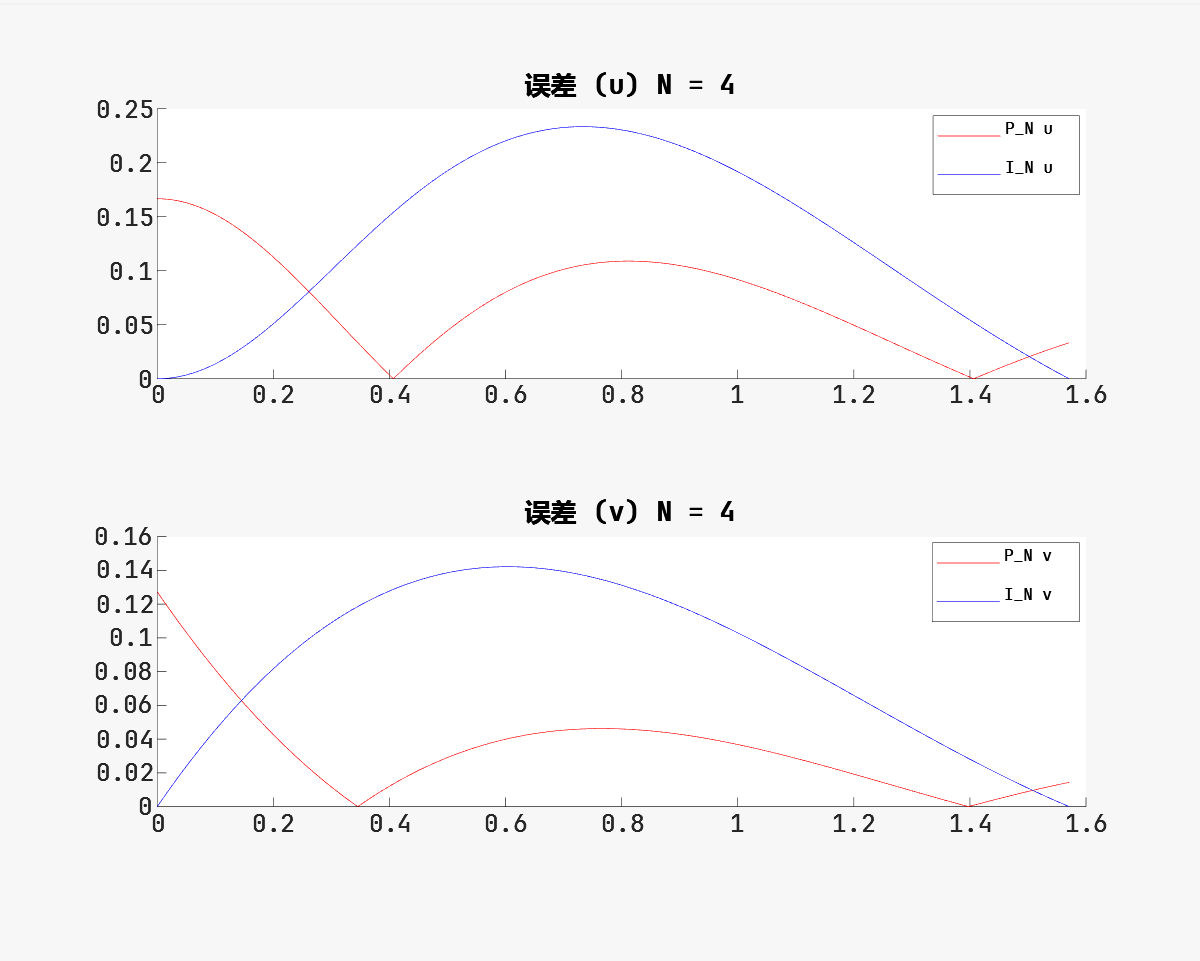
\includegraphics[width=0.8\textwidth]{figure/error_04.png}
			\caption{$N=4$ 时误差对比图(上图为 $u(x)$ 的逼近误差, 下图为 $v(x)$ 的逼近误差)}
		\end{figure}

		\begin{figure}[htbp]
			\centering
			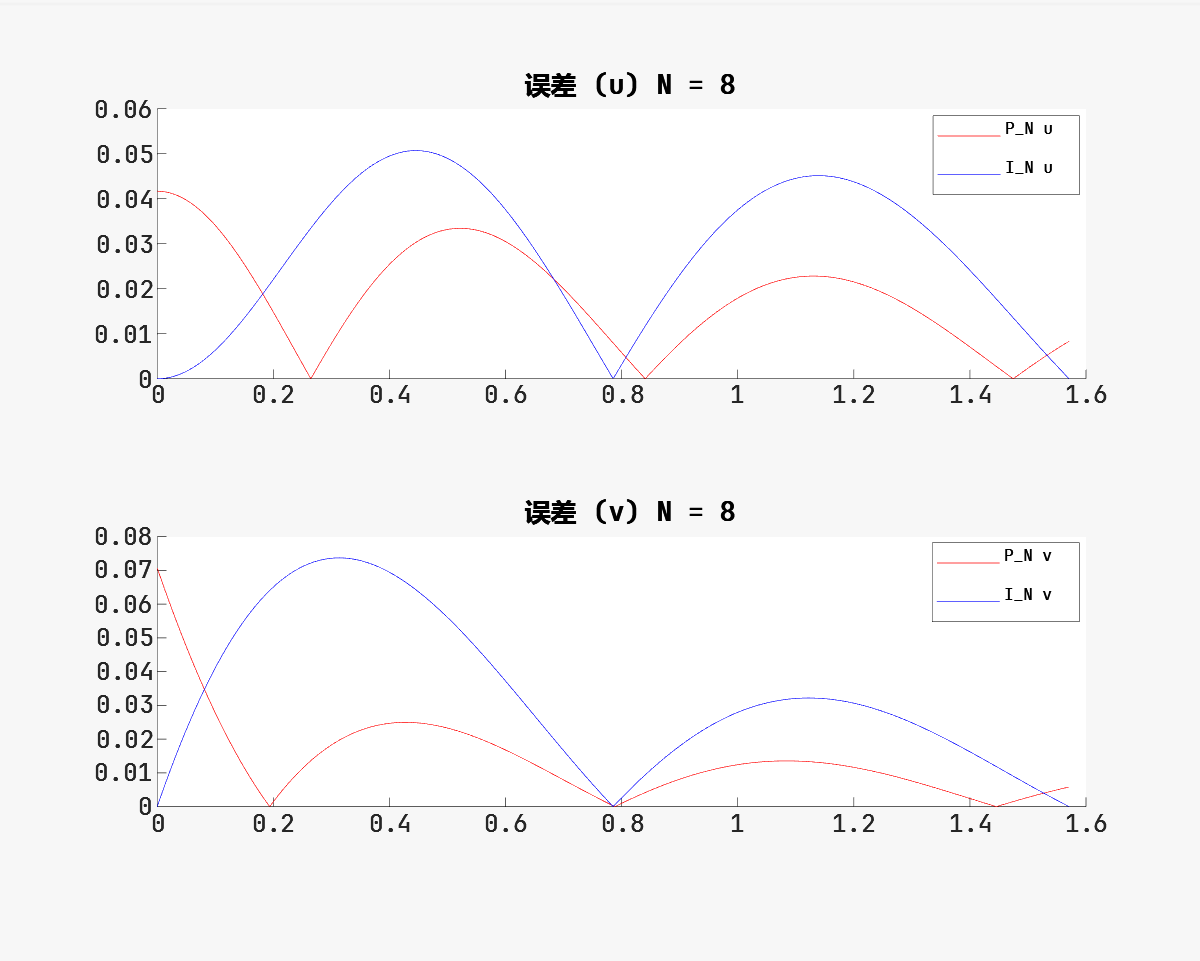
\includegraphics[width=0.8\textwidth]{figure/error_08.png}
			\caption{$N=8$ 时误差对比图}
		\end{figure}

		\begin{figure}[htbp]
			\centering
			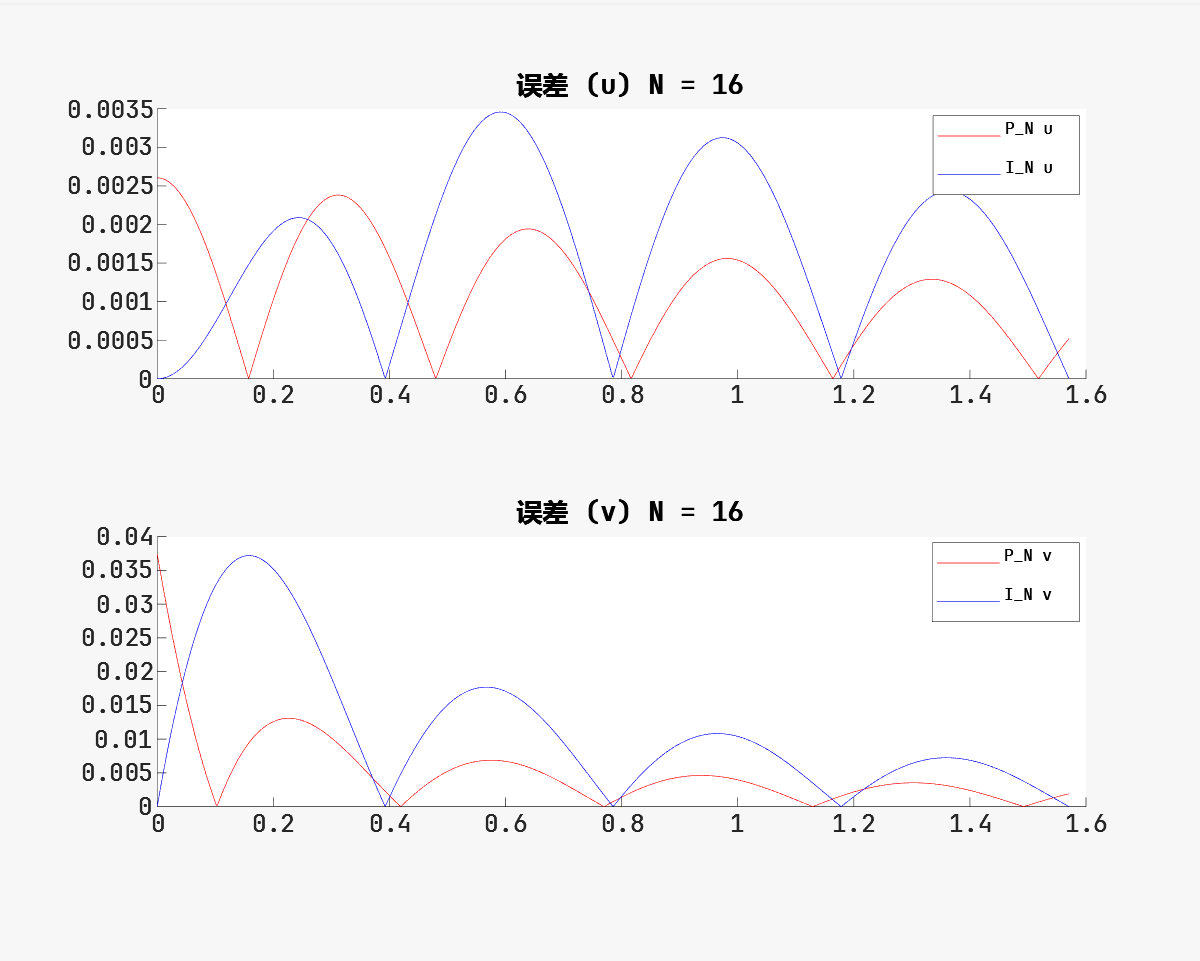
\includegraphics[width=0.8\textwidth]{figure/error_16.png}
			\caption{$N=16$ 时误差对比图}
		\end{figure}

		\begin{figure}[htbp]
			\centering
			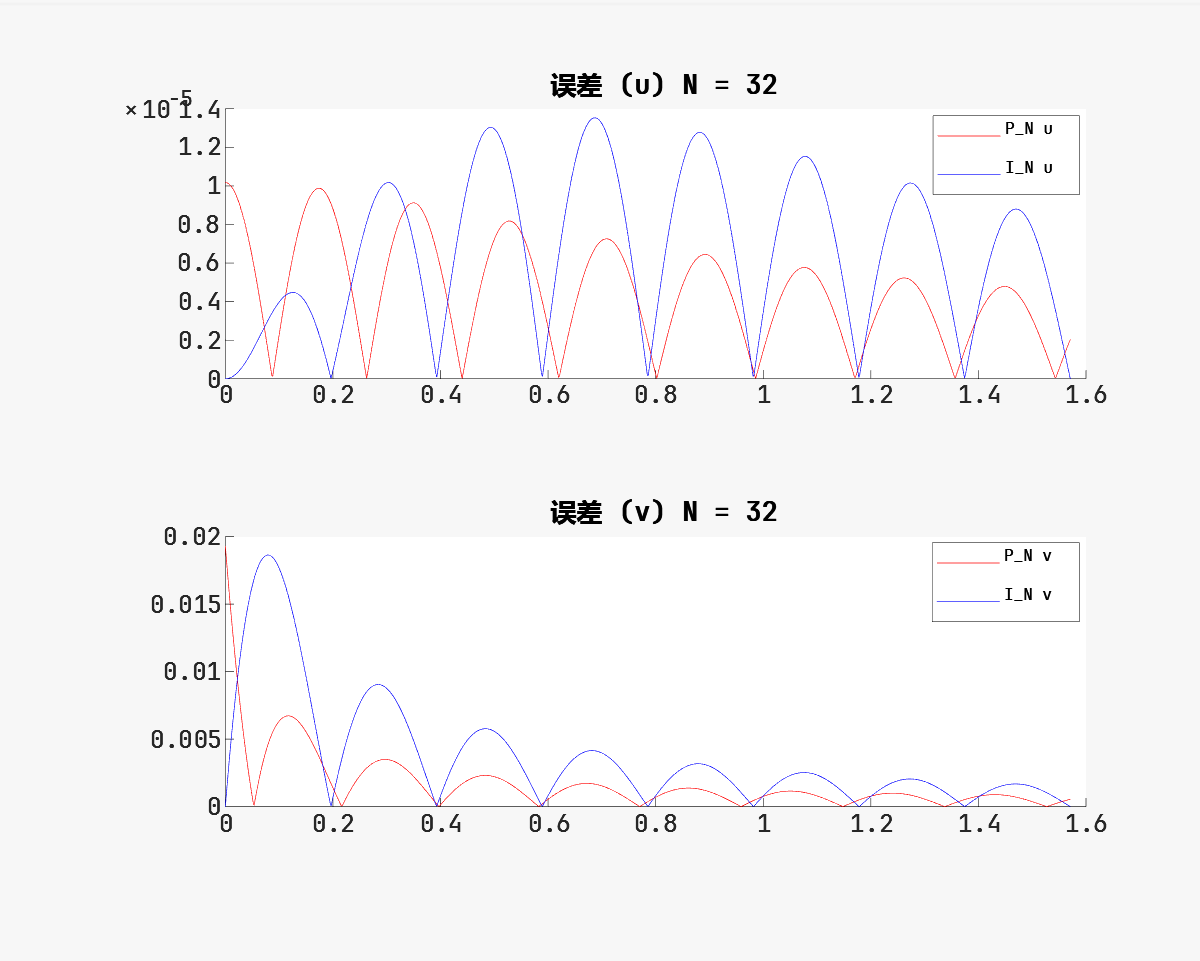
\includegraphics[width=0.8\textwidth]{figure/error_32.png}
			\caption{$N=32$ 时误差对比图}
		\end{figure}

		\begin{figure}[htbp]
			\centering
			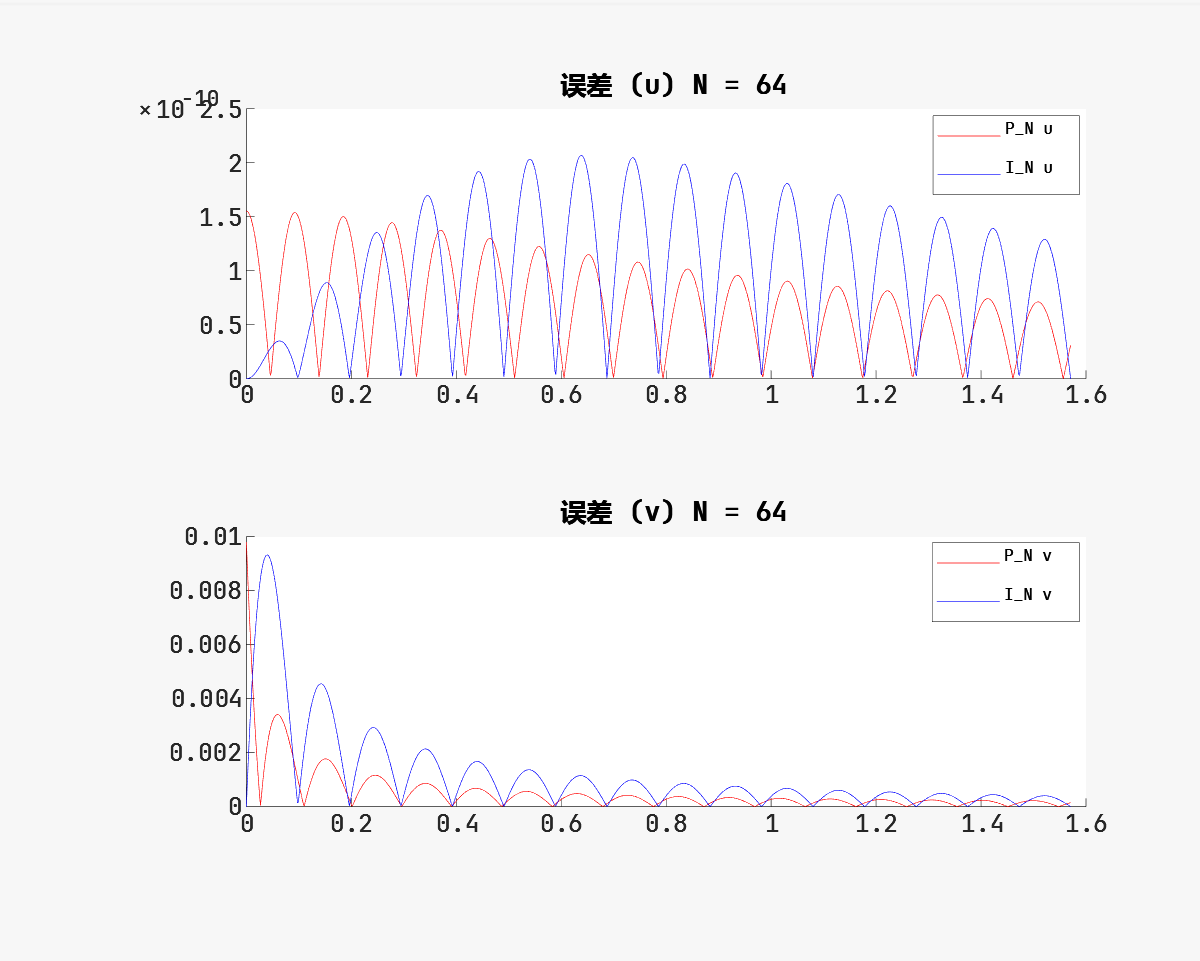
\includegraphics[width=0.8\textwidth]{figure/error_64.png}
			\caption{$N=64$ 时误差对比图}
		\end{figure}

\end{document}
